\documentclass[12pt]{article}
\usepackage{amsmath}
\usepackage{graphicx}
\usepackage{hyperref}
\usepackage{geometry}
\usepackage{cite}
\usepackage{cleveref}
\usepackage{listings}
\usepackage{xcolor}

\lstset{ 
    language=Python, 
    basicstyle=\ttfamily\footnotesize, 
    keywordstyle=\color{blue}, 
    commentstyle=\color{gray}, 
    stringstyle=\color{red}, 
    numbers=left, 
    numberstyle=\tiny\color{gray}, 
    stepnumber=1, 
    numbersep=10pt, 
    backgroundcolor=\color{lightgray!20}, 
    frame=single, 
    rulecolor=\color{black}, 
    breaklines=true, 
    breakatwhitespace=false, 
    showspaces=false, 
    showstringspaces=false, 
    showtabs=false, 
    tabsize=4, 
    captionpos=b
}


\geometry{a4paper, margin=1in}

\title{Image Compression Using Singular Value Decomposition}
\author{Shantanu Sinha}

\date{\today}

\begin{document}

\maketitle

\section{Introduction}

Image compression is an essential technique in digital photography, web development, and data storage, aiming to reduce image file sizes without significantly compromising quality. Singular Value Decomposition (SVD) is a powerful linear algebra method that can be effectively used for this purpose. This project explores the application of SVD in compressing images.

Research in image compression indicates that SVD provides an optimal approach to approximating and compressing images by reducing the rank of the image matrix. A paper in IEEE's Transactions on Acoustics, Speech, and Signal Processing \cite{IEEE_SVD} demonstrates how SVD can decompose an image matrix into singular vectors and values, which can then be truncated for compression.

In this report, we focus on compressing a 3-channel colour image represented by a matrix \(A\) of size \(m \times n\) (per channel), where each element \(a_{ij}\) corresponds to a pixel's intensity. Our goal is to use SVD to compress this image while maintaining acceptable quality. The method discussed here is based on Strang's \textit{Introduction to Linear Algebra} \cite{strang2006linear} and the algorithm described in the aforementioned IEEE paper \cite{IEEE_SVD}.




\section{SVD Compression Overview}
SVD's are a factorization method to decompose a matrix into three simpler matrices. In general form: SVD decomposes a matrix \(A\) into three matrices: \(A = U \Sigma V^T\). Once this decomposition is complete, essential features are meant to be retained, so the singular values in \(\Sigma\) (diagonal matrix with singular values) are sorted in descending order, and the largest values tend to be the most important values, or salient features of the image data. Then we need to truncate these values choosing some "k" most important values, and their corresponding vectors, which means we have a matrix \(A_k\) that is the approximate equivalent matrix of \(A\). In the case of image compression this truncated matrix will be a compressed version of the original image, ensuring the most important features of the image are kept.


\subsection{Performing SV Decomposition on the Image Matrix}
The first step is to decompose the matrix \(A\) of size \(m \times n\) into three matrices \(U\), \(\Sigma\), and \(V^T\) such that:
\[
A = U \Sigma V^T
\]
where:
\begin{itemize}
    \item \(U\) is an \(m \times m\) orthonormal matrix,
    \item \(\Sigma\) is an \(m \times n\) diagonal matrix with singular values,
    \item \(V^T\) is an \(n \times n\) orthonormal matrix.
\end{itemize}

\subsubsection{Steps to Find \(U\), \(\Sigma\), and \(V\)}

\begin{enumerate}
    \item Compute \(A^T A\) and \(A A^T\)

    \item Find the Singular Values (\(\sigma_i\)).. 
    
    \begin{enumerate}
    \item \textbf{Compute the eigenvalues of \(A^T A\)}:
    \[
    A^T A v_i = \lambda_i v_i
    \]
    where \(\lambda_i\) are the eigenvalues and \(v_i\) are the corresponding eigenvectors.

    \item \textbf{Compute the singular values}:
    \[
    \sigma_i = \sqrt{\lambda_i}
    \]
    Arrange the singular values in descending order: \(\sigma_1 \geq \sigma_2 \geq \cdots \geq \sigma_r \geq 0\), where \(r = \min(m, n)\).
    \end{enumerate}


    \item Find the Right Singular Vectors (\(V\)).

    \begin{enumerate}
    \item \textbf{Solve the eigenvalue problem}:
    \[
    A^T A v_i = \lambda_i v_i
    \]
    where \(v_i\) are the eigenvectors corresponding to the eigenvalues \(\lambda_i\).

    \item \textbf{Form the matrix \(V\)}:
    Stack the eigenvectors \(v_i\) as columns to form an \(n \times n\) matrix and normalize the vectors to form the orthonormal matrix \(V\):
    \[
    V = [v_1, v_2, \ldots, v_n]
    \]
    \end{enumerate}


    \item Using the computed right singular vectors \(V\) and singular values \(\sigma_i\), compute the left singular vectors (\(U\)):

    \begin{enumerate}
    \item For each \(v_i\), compute:
     \[
     u_i = \frac{A v_i}{\sigma_i}
     \]
     where \(\sigma_i\) is the corresponding singular value.

    \item \textbf{Form the matrix \(U\)}:
    Stack the eigenvectors \(u_i\) as columns to form an \(m \times m\) matrix and normalize the vectors to get the orthonormal matrix \(U\):
    \[
    U = [u_1, u_2, \ldots, u_m]
    \]
    \end{enumerate}


    \item Finally, we construct the Diagonal Matrix (\(\Sigma\)), where \(\Sigma\) is an \(m \times n\) diagonal matrix where the positive singular values \(\sigma_i\) are placed on the main diagonal, and zeros elsewhere:
    \[
    \Sigma = 
    \begin{pmatrix}
    \sigma_1 & 0 & \cdots & 0 \\
    0 & \sigma_2 & \cdots & 0 \\
    \vdots & \vdots & \ddots & \vdots \\
    0 & 0 & \cdots & \sigma_r \\
    0 & 0 & \cdots & 0 \\
    \vdots & \vdots & \ddots & \vdots \\
    0 & 0 & \cdots & 0
    \end{pmatrix}
    \]

\end{enumerate}


\subsection{Truncating the SVD Components}

To truncate the SVD components for compression, we select the top \(k\) singular values from \(\Sigma\) and their corresponding vectors in \(U\) and \(V^T\). This results in matrices \(U_k\), \(\Sigma_k\), and \(V_k^T\). The truncated SVD is given by:
\[
A_k = U_k \Sigma_k V_k^T
\]
where \(U_k\) is \(m \times k\), \(\Sigma_k\) is \(k \times k\), and \(V_k^T\) is \(k \times n\).

\subsection{Reconstructing the Compressed Image}
Using the truncated matrix, we can re-form the compressed image matrix \(A_k\).
\[
A_k = U_k \Sigma_k V_k^T
\]

This matrix \(A_k\) approximates the original image matrix \(A\) with reduced dimensionality. It retains the top \(k \) most significant entires which constitute the salient features of the image.

\section{Results}

To demonstrate the process and provide a proof of concept, an experiment was conducted using Python. In this experiment, a color image was subjected to the SVD compression algorithm, truncating the matrices to retain the top \(k\) singular values. The variations in storage requirements and image quality as a function of \(k\) were analyzed. The detailed implementation of the code is available on a {GitHub Repository}\footnote{\href{https://github.com/5han7anu-S/SVD_Compression}{https://github.com/5han7anu-S/SVD\_Compression}} and included in the appendix of this report.

As demonstrated in \autoref{fig:results}, the reconstructed image begins to resemble the original image fairly early in the compression process. When retaining only 25 singular values (across three color channels, totaling 75 elements), the image has already started to appear very similar to the original with only slight qualatative fuzziness. Further increasing the value of \( k \) enhances the sharpness of the image, but it is evident that the bulk of the information in this image can be approximated by only a few features. By \( k = 50 \), the reconstructed image becomes virtually indistinguishable from the original, all while only requiring 2.31\% of the information in the original image. From this, it is evident that SVD can be an effective tool for image compression.

\begin{figure}[h]
    \centering
    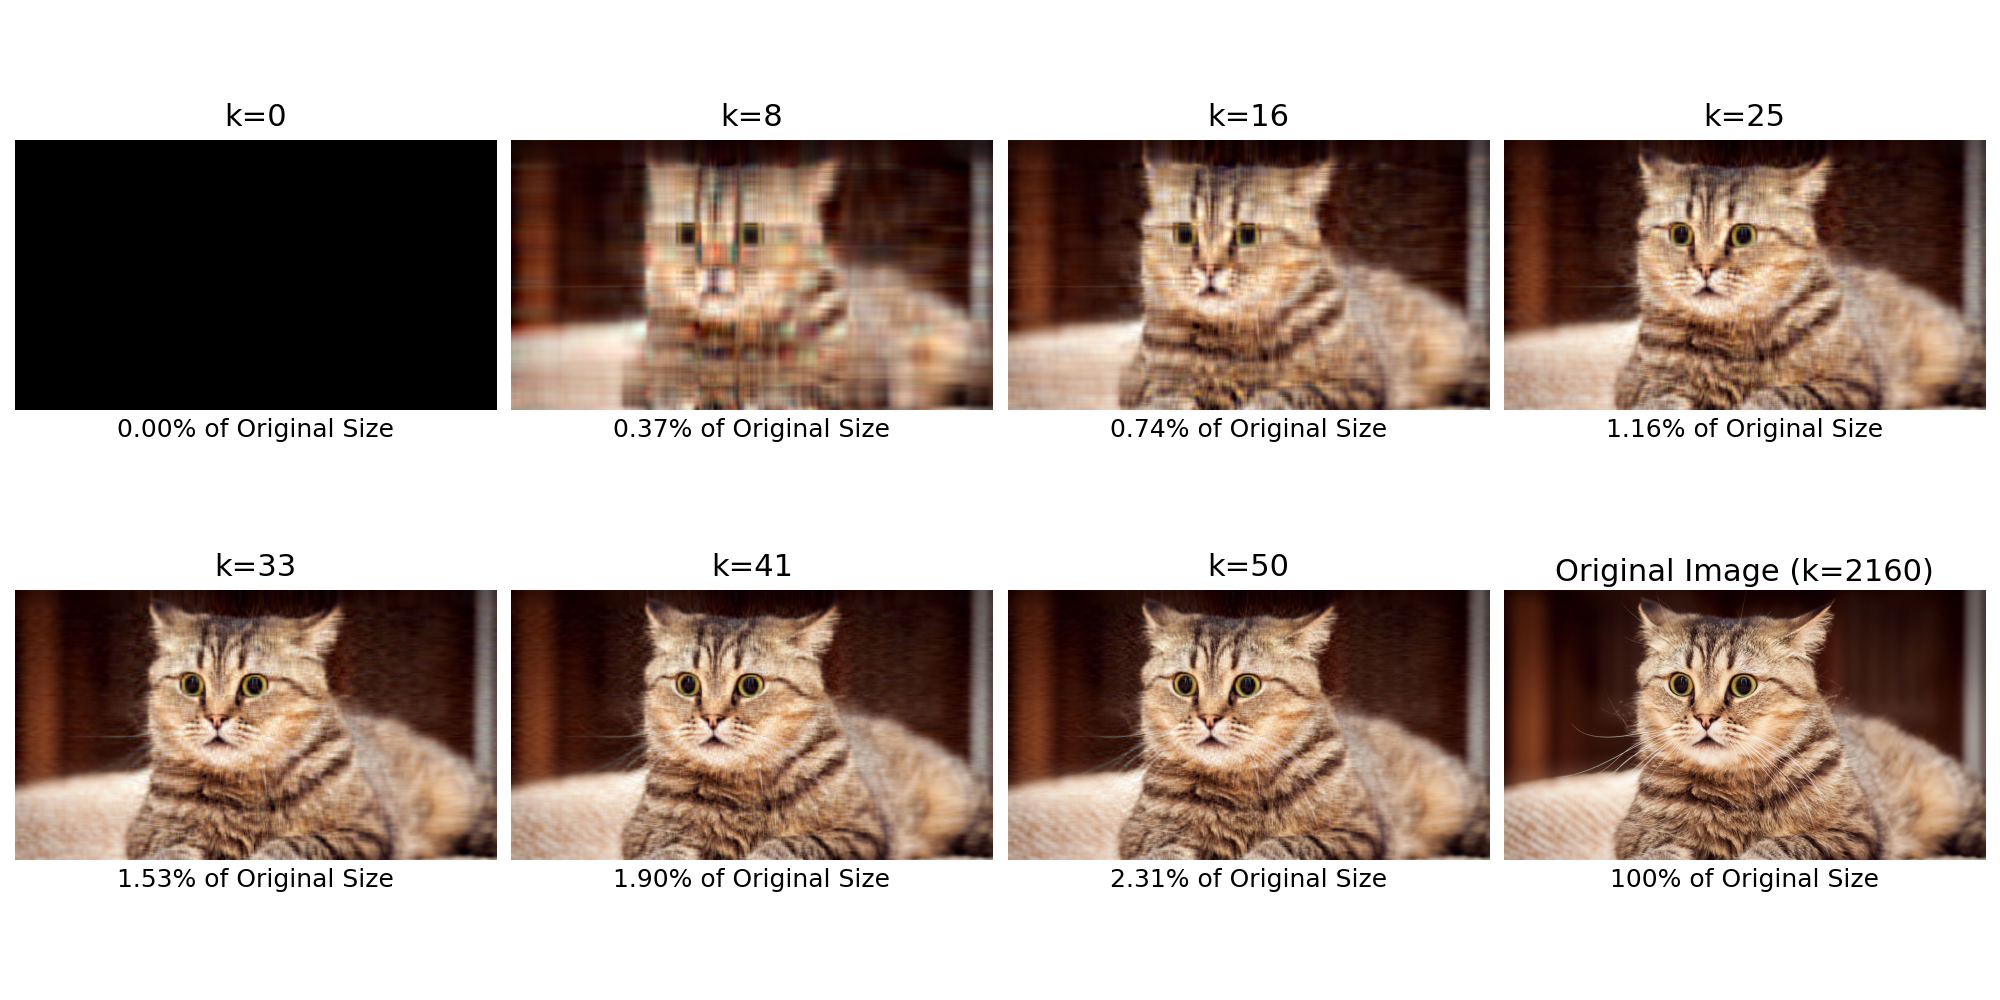
\includegraphics[width=\textwidth]{results.png}
    \caption{Reconstructed images using different values of \( k \).}
    \label{fig:results}
\end{figure}

\section{Conclusion}
Using SVD for image compression, we reduced the image size significantly. For \(k\) = 50, we are still achieving a compression ratio of approximately 50:1 while still retaining most of the quality. This method effectively preserves the essential features of the original image while significantly reducing the storage requirement. The choice of \(k\) allows control over the balance between compression and image quality, and further work could be done in determining an ideal value of \(k\) for optimum trade-off between reconstruction error and compression. However, while certainly a versatile tool, computing the SV Decomposition is computationally expensive and so it isn't used in most major compression algorithms which opt for something computationally cheaper.

\bibliographystyle{plain} % or any other style you prefer
\bibliography{citations.bib}


\pagebreak

\appendix
\section{Appendix:}

\begin{lstlisting}[language=Python, title={Python Code for SVD Compression}]

import numpy as np
import matplotlib.pyplot as plt
from PIL import Image
from scipy.linalg import svd

def reconstruct_image(U, S, Vt, k):
    """
    Reconstruct an image using Singular Value Decomposition (SVD) components.

    Parameters:
    - U, S, Vt: SVD components of the original image
    - k: Number of singular values to retain for each channel

    Returns:
    - reconstructed_image: 3D numpy array (compressed color image) in uint8 format
    """
    reconstructed_image = np.zeros((U[0].shape[0], Vt[0].shape[1], 3), dtype=np.float32)
    
    for i in range(3):
        Uk = U[i][:, :k]
        Sk = np.diag(S[i][:k])
        Vtk = Vt[i][:k, :]
        reconstructed_image[:, :, i] = np.dot(Uk, np.dot(Sk, Vtk))
    
    # Clip values for valid rgb range
    reconstructed_image = np.clip(reconstructed_image, 0, 255).astype(np.uint8)
    
    return reconstructed_image


def calculate_compression_percentage(U, S, Vt, k):
    """
    Calculate the compression percentage of the image.

    Parameters:
    - U, S, Vt: SVD components of the original image
    - k: Number of singular values to retain
    - original_size: Size of the original image in bytes

    Returns:
    - compression_percentage: Compression percentage relative to the original size
    """

    compressed_size = sum([U[i][:, :k].size + S[i][:k].size + Vt[i][:k, :].size for i in range(3)])
    original_size = sum ([U[i].size + S[i].size + Vt[i].size for i in range (3)])

    return ((compressed_size / original_size)) * 100

def load_image(image_path):
    # Load the image using Pillow and convert to RGB
    pil_image = Image.open(image_path).convert('RGB')
    return np.array(pil_image)

if __name__ == "__main__":
    image_path = 'images/cat.png'
    image = load_image(image_path)

    # Perform SVD on each channel
    U = []
    S = []
    Vt = []
    for i in range(3):
        u, s, vt = svd(image[:, :, i], full_matrices=False)
        U.append(u)
        S.append(s)
        Vt.append(vt)

    k_values = np.linspace(0, 50, 7, dtype=int)
    
    # Reconstruct with different k
    compressed_images = [reconstruct_image(U, S, Vt, k) for k in k_values]
    compression_percentages = [calculate_compression_percentage(U, S, Vt, k) for k in k_values]

    # Plot the original and compressed images
    fig, axes = plt.subplots(2, 4, figsize=(20, 10))
    plt.subplots_adjust(wspace=0.1, hspace=0.2)

    for i, (ax, k, comp_img, perc) in enumerate(zip(axes.flat[:-1], k_values, compressed_images, compression_percentages)):
        ax.imshow(comp_img.astype(np.uint8))
        ax.set_title(f'k={k}', fontsize=22, pad=10)
        ax.text(0.5, -0.1, f'{perc:.2f}% of Original Size', fontsize=18, ha='center', transform=ax.transAxes)
        ax.axis('off')

    axes[1, 3].imshow(image)
    axes[1, 3].set_title(f'Original Image (k={len(S[0])})', fontsize=22)
    axes[1, 3].text(0.5, -0.1, '100% of Original Size', fontsize=18, ha='center', transform=axes[1, 3].transAxes)
    axes[1, 3].axis('off')

    plt.tight_layout()
    plt.savefig("images/results.png")

    
\end{lstlisting}


\end{document}
